\chapter{Energia}

\section{Solução de Suprimento de Energia}

Considerando que o sistema radar possui o funcionamento em regime permanente, o dimensionamento da fonte de alimentação para o produto comercial foi realizado considerando os consumos energéticos da iluminação e dos componentes eletrônicos. Porém, devido às limitações de orçamento e recursos disponíveis, o dimensionamento do protótipo a ser construído foi realizado considerando o funcionamento do radar durante 3 horas por dia, para a alimentação das cargas mostradas na Figura \ref{fig30}.

\begin{figure}[H]
\centering 
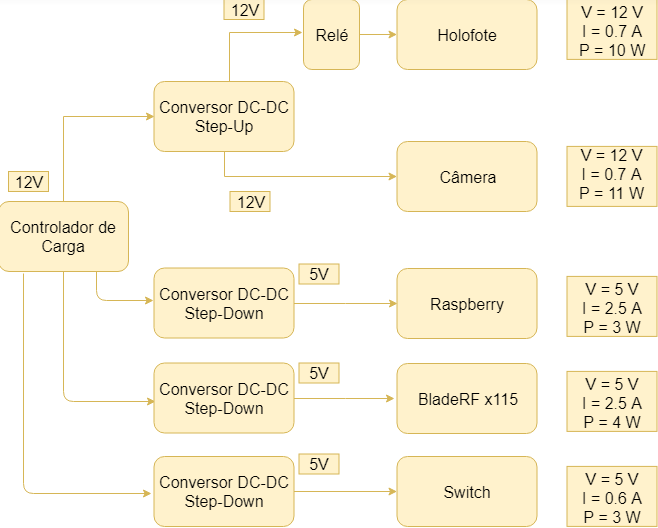
\includegraphics[scale=0.5]{pot}
\caption{\label{fig30}Diagrama de alimentação de energia pela geração fotovoltaica }
\end{figure}

A Figura \ref{fig30} representa as cargas que devem ser alimentadas pela geração fotovoltaica assim como os conversores adotados para garantir que chegue a tensão correta para as cargas. O conversor \textit{Step-up} vai garantir que chegue os 12V nas cargas que necessitam de 12V e o conversor \textit{Step-down} vai diminuir o valor da tensão para 5V para as cargas que precisam de apenas 5V, funcionando como uma proteção as cargas.

A Figura \ref{fig31} representa a integração entre o escopo da engenharia de energia e a engenharia eletrônica dentro do projeto do radar. Os itens em amarelo representa o escopo de energia e os itens em azul representa o escopo de eletrônica.

\begin{figure}[H]
\centering 
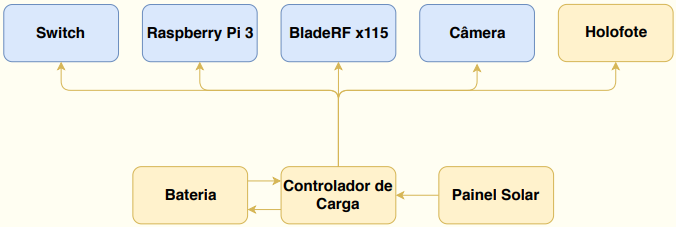
\includegraphics[scale=0.6]{energronica}
\caption{\label{fig31}Diagrama de integração energia-eletrônica.}
\end{figure}

\section{Recurso Solar}

O projeto será instalado e testado inicialmente no Campus FGA da Universidade de Brasília, localizado no Gama, cujas as coordenadas são: 15º59’24”S e 49º02’43”O. A partir das coordenadas, é possível verificar os valores de irradiação solar diária média do local mais próximo na base de dados do CRESESB \cite{solar}.

Pretende-se que o radar seja instalado em diversas regiões do Brasil, em trechos de estradas perigosas, com isso recomenda-se um estudo de caso sobre a irradiação solar diária em cada região que o radar for implantado, para se obter um melhor rendimento solar do sistema fotovoltaico. 
\begin{figure}[H]
\centering
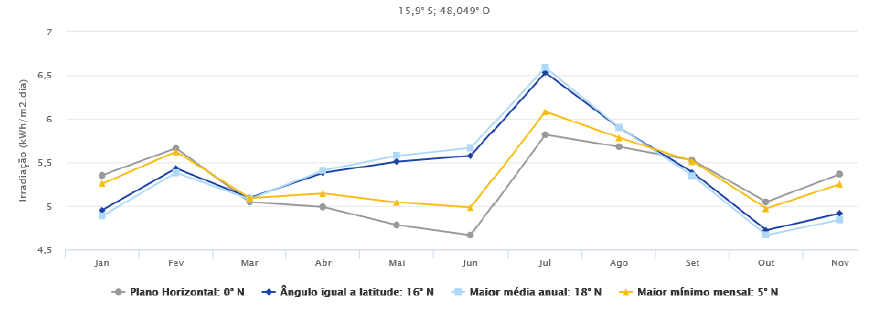
\includegraphics[scale=0.5]{grafico}
\caption{Irradiação Solar Gama-Brasília-DF \cite{solar}.}
\label{fig:grafico}
\end{figure}

Verifica-se na Figura \ref{fig:tabela} que a maior média anual de Brasília é de 5,44 $KWh/m^2dia$, que é um ótimo valor comparado a outras regiões. Aliado á baixa nebulosidade e pluviosidade, o Distrito Federal é um local ideal para implantação de sistemas fotovoltaicos.

\begin{figure}[H]
\centering
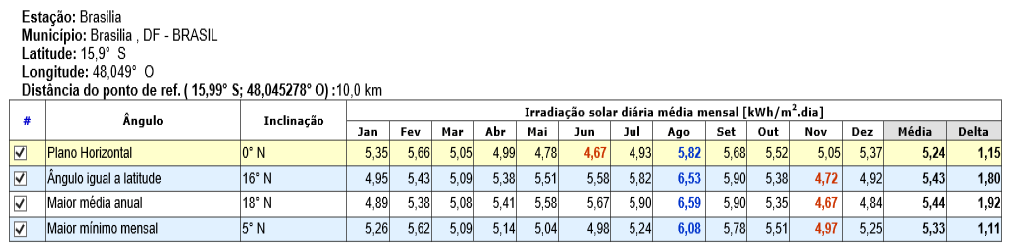
\includegraphics[scale=0.5]{tabela}
\caption{Valores de irradiação solar média \cite{solar}.}
\label{fig:tabela}
\end{figure}

\subsubsection{Definição da inclinação do painel}

A inclinação dos módulos fotovoltaicos instalados é determinado de acordo com a latitude do local. A localização em questão possui os dados de latitude iguais a $15^{\circ}59’24”$ S. Analisando então os dados de irradiação solar fornecidos pelo Centro de Referência em Energia Solar e Eólica - CRESESB \cite{solar}, temos que, na região de Brasília, o ângulo considerado é o ângulo de $15^{\circ}$. Dessa forma, devido à proximidade dos ângulos e os dados obtidos, será utilizado neste projeto o ângulo de inclinação de $15^{\circ}$ para o módulo fotovoltaico.

Com isso, será considerado para os  cálculos os dados que  trata da radiação global no plano inclinado  igual à latitude para a localidade.
 
 
\section{Dimensionamento da Placa Fotovoltaica}

O dimensionamento do painel fotovoltaico levou em consideração o suprimento de toda a carga do sistema radar, como mostra a Tabela \ref{tab24}, que representa a carga a ser alimentada pela geração fotovoltaica. 

\begin{table}[H]
\caption{Cargas a serem alimentadas pela geração solar}\label{tab24}
\begin{tabular}{|c|c|c|c|}
\hline
\multicolumn{4}{|c|}{Consumo de energia durante 24 horas de funcionamento do radar}                                                 \\ \hline
Dispositivos & Potência & Tempo de consumo diário & Consumo total diário \\ \hline
Raspberry Pi 3  & 30W  & 24  & 720Wh  \\ \hline
Câmera & 8.4W  & 12 & 100.8Wh \\ \hline
BladeRFmx115 & 30W  & 24 & 720Wh \\ \hline
LED       & 8.4W &  12 & 100.8Wh  \\ \hline
Switch       & 3W &  24 & 72Wh \\ \hline
Total & 84W & - & 1713.6Wh \\ \hline

\end{tabular}
\end{table}
\FloatBarrier

Considerando o funcionamento do radar em um período de 24 horas e que necessariamente a \textit{BladeRF}, \textit{Raspberry} e \textit{Switch} precisariam funcionar durante as 24 horas e apenas a iluminação e a câmera funcionaria em um período médio de 12 horas. O consumo total da carga é 1713.6 Wh e a potência mínima dos painéis de geração seria 453.33 Wp.

A Tabela \ref{tab6} apresenta o consumo das cargas durante um período de 3 horas.

\begin{table}[H]

\caption{\label{tab6}Consumo das cargas durante um período de 3 horas.}
\begin{tabular}{|c|c|c|c|} 

\hline
Dispositivos             & Potência         & Tempo de consumo diário & Consumo total diário \\ \hline
Raspberry Pi 3  & 30W  & 3 horas          & 90Wh    \\ \hline
Câmera & 8.4W  &   1.5 horas        & 12.6Wh \\ \hline
BladeRFmx115 & 30W  & 3 horas         & 90Wh \\ \hline
LED       & 8.4W &  1.5 horas & 12.6Wh    \\ \hline
Switch       & 3W &  3 horas & 9 Wh    \\ \hline
Total & 84W & - & 214.2 Wh \\ \hline

\end{tabular}
\end{table}
\FloatBarrier

Para este trabalho será considerado para os cálculos e compra de materiais uma autonomia de 3 horas para o funcionamento do radar. Com isso para a  \textit{BladeRF}, \textit{Raspberry} e \textit{Switch} será considerado a autonomia total de 3 horas e para a iluminação e câmera será considerado 1.5 horas. Com essas considerações temos uma necessidade de suprir uma carga de 214.2 W e a Eq. \ref{potenciamin} define a potência mínima.
\begin{equation}
    Pmin = \frac{Potencia\ \ total}{HSP \times FS} =\frac{214.2}{(4,72)(0,8)} = 56,73 Wp
    \label{potenciamin}
\end{equation}

Onde HPS é horas de sol pleno e FS é rendimento dos componentes, bateria, controlador e perdas nos fios.

A variável HSP é determinada por meio do valor da radiação do mês que apresentou o menor índice, este valor pode ser observado na figura apresentada com os dados do CRESESB \cite{solar} na irradiação global no plano inclinado igual á latitude para a localidade. A menor radiação observada para a localidade foi no mês de novembro no valor de 4,72 $kWh/m^2$dia. 
 
De acordo com os cálculos acima serão instalados dois painéis em paralelo de 45 Wp, fabricado pela \textit{Kyocera}, com uma potência instalada de 90 Wp. Os dois painéis em paralelo serão ligados em um único controlador de carga, não tendo empecilho  por se tratar de dois painéis de mesma capacidade e mesmo fabricante. 


\begin{figure}[H]
\centering
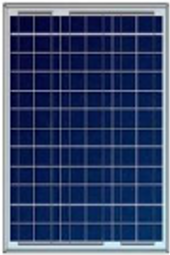
\includegraphics[scale=0.6]{placa}
\caption{Representação do painel fotovoltaico 45 W.}
\end{figure}

\section{Dimensionamento da Bateria}

Componente fundamental do sistema autônomo, pois como o nome já disse, ele precisa ser totalmente independente de qualquer outra fonte primária de energia elétrica e a escolha adequada da capacidade da bateria é de muita importância, pois ela garante a continuidade do fornecimento da energia elétrica mesmo em condições adversas para a geração fotovoltaica, exemplificando, durante o período noturno e nos dias de chuva \cite{alan}.
\begin{itemize}

 \item\textbf{Dimensionamento do produto comercial}
\end{itemize}
Levando em consideração a carga total do sistema 84W e considerando dias nublados e períodos em que não há irradiação, a bateria deve ser capaz de alimentar o sistema por 24 horas.
Então, a energia diária consumida é realizada com base no consumo diário de cada dispositivo e já considerado seu dispositivo de proteção, apresentado na Tabela \ref{tab24}.

Com os valores observados na Tabela \ref{tab24}, é possível calcular a capacidade do sistema de acumulação a partir da Eq. \ref{eq:capacidade} \cite{alan}:

\begin{equation}
    C_{Bat} = \frac{CB \times N}{Pd \times Ef}
    \label{eq:capacidade}
\end{equation}




Onde $C_{Bat}$ é a capacidade total da bateria, $CB$ é a energia diária solicitada pelas cargas por dia em Ah (ampere hora), $N$ é o número de dias de autonomia, $Pd$ é a máxima profundidade de descarga da bateria (tipicamente varia de 50 a 80\%) e $Ef$ é a eficiência da bateria.

Sendo 12 V a tensão padrão das baterias comerciais, obtemos o valor de consumo diário de 151.2 Ah. Fixando-se um valor de $N$ igual a 1 dia e um valor de $Pd$ igual a 70\% e o valor da eficiência como 90\% obtém-se os valores de capacidade de $CB = 240 Ah$. 


Dessa forma, optou-se por uma bateria de 12V da marca \textit{Heliar Freedom} com uma capacidade de 185 Ah associada em paralelo com outra bateria da mesma marca com capacidade de 70 Ah. Na Figura \ref{fig:bateria} serão apresentadas a bateria escolhidas por possuírem os melhores parâmetros de preço e qualidade.


\begin{figure}[H]

    \centering
      \begin{subfigure}{0.45\textwidth}
        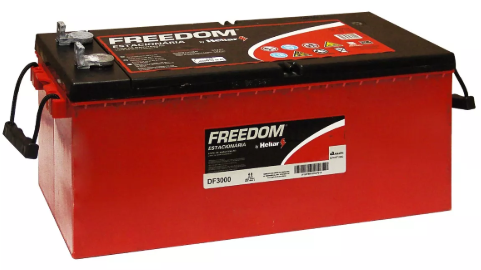
\includegraphics[width=\textwidth]{bateria185}
        \caption{Bateria Heliar Freedom de 185Ah.}
      \end{subfigure}
      \hfill
      \begin{subfigure}{0.35\textwidth}
        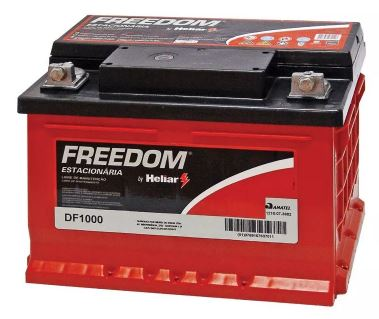
\includegraphics[width=\textwidth]{bateria70}
        \caption{Bateria Heliar Freedom de 70Ah.}
      \end{subfigure}
    \caption{Baterias escolhidas para o sistema de armazenamento.}
    \label{fig:bateria}
\end{figure}


    \begin{itemize}
        \item \textbf{Dimensionamento do protótipo}
    \end{itemize}
    
    Em termos de armazenamento de energia, o protótipo possuirá duas baterias da marca \textit{Unipower} com capacidade de 7 Ah.Tendo em vista que a demanda de corrente do projeto é de 7 A, o protótipo possuirá autonomia de 2 horas. A Figura \ref{fig:bateriaunip} ilustra a bateria utilizada para o sistema de armazenamento.
    

\begin{figure}[H]
\centering
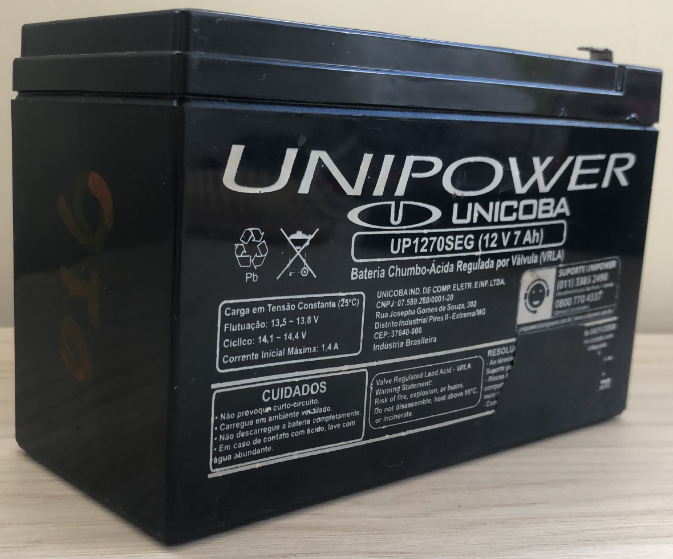
\includegraphics[scale=0.2]{bateriaunip.PNG}
\caption{Bateria Heliar Freedom de 70Ah escolhida para o Sistema de Armazenamento.}
\label{fig:bateriaunip}
\end{figure}

\section{Dimensionamento do Controlador de Carga}

Para o correto dimensionamento do controlador de carga é preciso conhecer as máximas correntes às quais ele será submetido, tanto do lado dos painéis geradores quanto do lado das cargas. A corrente máxima, circula no lado dos painéis geradores e possui valor de 30,4 A.

Portanto, foi selecionado o controlador de carga da marca \textit{Charge Controller} com limite de carga e descarga de 40 A. Na Figura \ref{fig:control}, será apresentado o controlador de carga escolhido.

\begin{figure}[H]
\centering
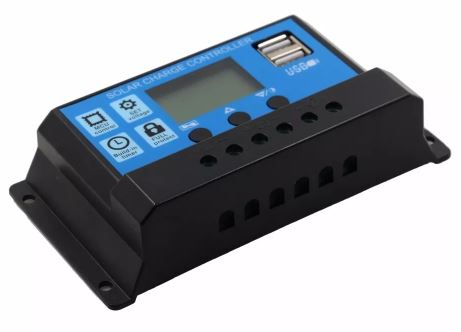
\includegraphics[scale=0.4]{control}
    \caption{Controlador de carga da marca \textit{Charge Controller} com limite de 10 A escolhida para o Sistema de Proteção.}
\label{fig:control}
\end{figure}


Para o protótipo, um controlador de carga da mesma marca e capacidade de 30 A será utilizado.

\section{Dimensionamento da Iluminação}

Com o objetivo de alertar o motorista quando houver outro veículo em sentido contrário, a solução para o subsistema iluminação foi que cada totem terá um holofote com lâmpada LED da marca SR, onde a fonte de alimentação é um barramento infinito alimentado pela bateria, onde a energia é transferida do barramento para a luminária através de um condutor conectado com um relé. 

Tendo em vista o custo-benefício, foi escolhido para a iluminação um holofote LED com função RGBW para o subsistema iluminação. Na Figura \ref{fig:holofotergbw} será apresentada a luminária escolhida.

\begin{figure}[H]
\centering
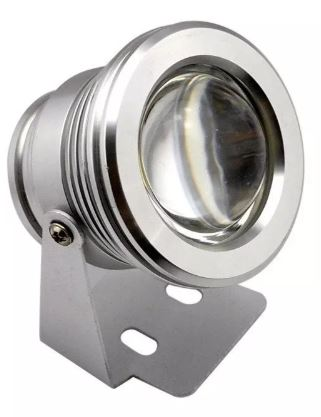
\includegraphics[scale=0.3]{holofotergbw}
\caption{Lúminária LED RGBW}. 
\label{fig:holofotergbw}
\end{figure}



Na Tabela \ref{tab:luminaria} serão apresentados os dados técnicos da luminária escolhida.

    \begin{table}[H]
    

\begin{tabular}{|c|c|c|c|c|c|c|}
\hline
\multicolumn{7}{|c|}{Dados da luminária escolhida}                                                 \\ \hline
Marca             & Tensão         & Corrente & Potência & Altura & Largura & Comprimento \\ \hline
Panabraks  & 12V  & 0.83          & 10W   & 10.3cm & 7.2cm & 7.2cm \\ \hline

\end{tabular}
    \caption{\label{tab:luminaria}Tabela de dados da luminária}
\end{table}


\section{Dimensionamento dos dispositivos de proteção}

\begin{itemize}
    \item \textbf{Conversor DC-DC}
\end{itemize}
O conversor DC/DC  é um conversor de tensão que converte um nível de tensão inicial em outro secundário, regulando a tensão de saída em relação a uma tensão de entrada. Foi escolhido por causa da alta eficiência (perda típica de 12\% da potência de entrada) para fornecer a tensão que os componentes eletrônicos demandam. No projeto serão utilizados três conversores \textit{step-down} e um conversor \textit{step-up}.
    
Seu circuito é composto por uma chave (S), a qual permanece fechada por um tempo \textit{t.on} e aberta por um tempo \textit{t.off}, durante um tempo de chaveamento T. A chave está ligada a um filtro composto por um indutor (L) e um capacitor (C) , que têm a função de uniformizar os parâmetros de tensão que chegam à carga. Ocorre que, a chave não pode ser aberta se a corrente que passa por ela não for nula, pois causaria uma sobretensão no indutor. Com isso, utiliza-se um diodo de retorno (D), que proporciona um caminho para a corrente do indutor (iL) enquanto a chave estiver aberta. Na Figura \ref{fig:circuitostepdown} será apresentado o circuito do conversor DC-DC \cite{Amauri}.

\begin{figure}[H]
\centering
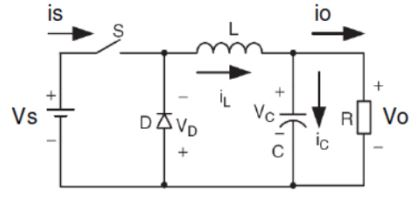
\includegraphics[scale=0.9]{circuitostepdown}
    \caption{Circuito elétrico do Conversor DC-DC \cite{Amauri}.}
\label{fig:circuitostepdown}
\end{figure}


Para dimensionar o conversor DC-DC adequado para a \textit{Raspberry} e a \textit{BladeRFx115}, dimensionamos a partir da tensão de entrada dos módulos, que tem como fonte a bateria de 12V a necessidade de uma tensão de saída ($V_0$) de 5V. Como a corrente que circulará na \textit{Raspberry} e na \textit{BladeRFx115} é 2,5A, o valor da resistência para cada conversor DC-DC será igual a $5=R \times 2,5$ sendo $R= 2 \Omega$. \cite{MSM}.

Para dimensionar o conversor do circuito do \textit{Switch}, possuímos a mesma tensão de entrada e saída. Porém, a corrente que circula nessa carga é de 0,6A. Logo, o valor da resistência será igual a $5=R \times 0.7$ sendo $R= 7,14 \Omega$.

Para o circuito da câmera e do holofote, a tensão de entrada também corresponde a tensão da bateria, de 12V e a tensão de saída ($V_0$) é 12.5V. Como a corrente que circulará no circuito em paralelo do holofote e da câmera é 1,4 A, o valor da resistência para cada conversor DC-DC será igual a $12,5=R \times 1,4$ sendo $R= 8,92 \Omega$.

Os Conversores DC/DC utilizados no circuito da \textit{Raspberry}, \textit{BladeRFx115}, \textit{Switch}, Holofote e Câmera são do modelo XL6019, suportam tensões de entrada de 6 a 40VDC, e consegue fornecer, de forma ajustável, uma tensão de 1,3 a 35V e uma corrente de até 5A, tendo um rendimento de 94\%. Na Figura \ref{fig:conversordc} será apresentado o Conversor DC-DC escolhido para o projeto.


\begin{figure}[H]
\centering
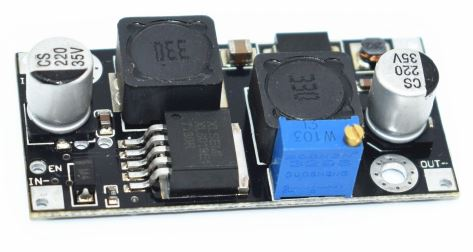
\includegraphics[scale=0.6]{conversordc}
    \caption{Conversor DC-DC modelo XL6019 escolhido para o sistema de proteção das cargas.}
\label{fig:conversordc}
\end{figure}
\FloatBarrier


\begin{itemize}

    \item \textbf{Relé}
    
\end{itemize}

O relé é um interruptor eletromecânico, se movimenta fisicamente com a passagem de corrente elétrica pelas espiras de sua bobina, criando assim um campo eletromagnético que atrai a alavanca responsável pela mudança do estado entre os contatos. Além disso, sabe-se que para energizar corretamente um relé, e ativar suas chaves internas, é necessário que uma corrente de intensidade mínima circule pela sua bobina. Sendo assim, deve-se aplicar uma tensão de determinado valor, que devido a resistência do enrolamento, permita que essa corrente circule pelos terminais da bobina. Os relés são especificados por sua de tensão nominal na bobina, a corrente máxima da chave e o valor de corrente que deve circular na bobina \cite{Braga}.

Para o projeto, foi escolhido o Módulo Relé 1 canal-5V com corrente típica de operação 15~20mA, com capacidade de 30VDC e 10A e tempo de resposta de 5-10ms. Na figura \ref{fig:rele} será apresentado o relé escolhido para o sistema de proteção do circuito da câmera.

\begin{figure}[H]
\centering
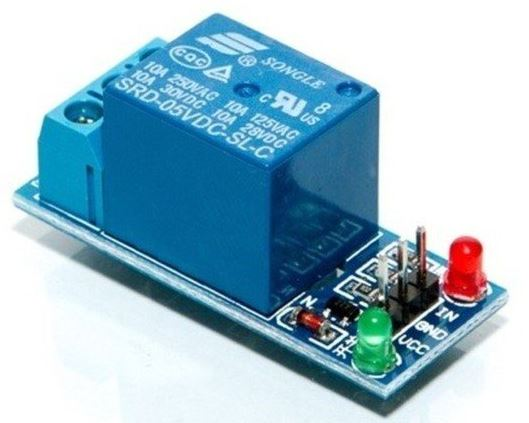
\includegraphics[scale=0.5]{rele}
    \caption{Módulo relé 1 canal-5V escolhido para o circuito de proteção da câmera.}
\label{fig:rele}
\end{figure}
\FloatBarrier

\subsection{Dimensionamento dos cabos}

A seção transversal do cabo deve ser dimensionada em função da corrente máxima de serviço que atravessa o cabo. De acordo com a norma europeia IEC 60364-7-712 \cite{instalacao} o cabo deve ser capaz de suportar 1,25 vezes a corrente de curto-circuito do gerador e estar protegido contra falhas de terra e curto-circuito. 

Neste projeto, os cabos deverão suportar, $I = 7A \times 1,25 = 8,75A$ do controlador de carga e a alimentação de carga. Por possuir quatro painéis ligados em paralelo e cada painel possui $I_{cc} = 3,04 A$ a corrente considerada para o dimensionamento foi $I = 12,6A \times 1,25 = 15,75 A$ entre o painel e o  controlador de carga, considerando a corrente de curto circuito do painel. $I = 7,3A \times 1,25 = 9,12 A$ entre a bateria e o controlador de carga. Outro ponto importante é a queda de tensão nos cabos que deve ser reduzida com o aumento da bitola, evitando uma queda de tensão significativa.

Considerando a ABNT NBR 5410 \cite{protecao}, o método de instalação B1 e que teremos dois condutores carregados um positivo e um negativo, e que a temperatura pode chegar a $60^{\circ}C$. O fator de correção a $60^{\circ}C$ será 0,50.  Dessa forma, será utilizado um condutor com seção de $4mm^2$ para toda a fiação que a corrente for até 16A ($32 \times 0.5 = 16A$) e a fiação do painel solar até o controlador de carga será utilizado um condutor de $6mm^2$, consegue suportar a corrente que o painel irá transmitir ao controlador de carga. 

O condutor de proteção será calculado a partir da seção dos condutores de fase do circuito, de acordo com a Tabela \ref{secao}.


\begin{table}[H]
 \centering
 \caption{\label{secao}Seção miníma dos condutores de proteção \cite{protecao}.}
% distancia entre a linha e o texto
 {\renewcommand\arraystretch{1.25}
 \begin{tabular}{ l l }
  \cline{1-1}\cline{2-2}  
    \multicolumn{1}{|p{4.133cm}|}{Seção miníma dos condutores de fase (mm²) \centering } &
    \multicolumn{1}{p{4.450cm}|}{Seção miníma dos condutores de proteção (mm²) \centering }
  \\  
  \cline{1-1}\cline{2-2}  
    \multicolumn{1}{|p{4.133cm}|}{S\textless = 16 \centering } &
    \multicolumn{1}{p{4.450cm}|}{S \centering }
  \\  
  \cline{1-1}\cline{2-2}  
    \multicolumn{1}{|p{4.133cm}|}{16\textless = S \textless = 35 \centering } &
    \multicolumn{1}{p{4.450cm}|}{16 \centering }
  \\  
  \cline{1-1}\cline{2-2}  
    \multicolumn{1}{|p{4.133cm}|}{S\textless = 35 \centering } &
    \multicolumn{1}{p{4.450cm}|}{$0,5 \times S$ \centering }
  \\  
  \hline

 \end{tabular} }
\end{table}

Considerando as espessuras dos condutores citadas acima, $4mm^2$ e $6mm^2$, os condutores de proteção (terra) serão de $4mm^2$.

\subsection{Dispositivos de proteção contra surtos}

Os dispositivos de proteção contra surtos (DPS) são importantes para proteger o sistema contra surtos elétricos provocados por descargas atmosféricas. Esses efeitos causam, por um período curto de tempo, uma elevação brusca na tensão nominal do sistema, com consequências muitas vezes devastadores, podendo causar surtos no sistema de energia e em sistemas de telecomunicações possuindo correntes que podem ultrapassar 200 kA \cite{surtos}.

Os DPS devem atender à IEC 61643-1 \cite{surtos} e ser selecionados com base no mínimo nas seguintes características: nível de proteção, máxima tensão de operação contínua, suportabilidade a sobretensões temporárias, corrente nominal de descarga e/ou corrente de impulso e suportabilidade à corrente de curto circuito.
 
 Para proteger o sistema contra os surtos citados anteriormente, existe diferentes classes de DPS para se adequar ao tipo de sistema, abaixo as principais diferenças entre as classes:
 
 \textbf{Classe I:} Os DPS  de Classe I permitem eliminar os efeitos diretos causados pelas descargas atmosféricas. 
 
\textbf{Classe II:} Os DPS são destinados a proteger os equipamentos elétricos contra sobretensão induzidas ou conduzidas (efeitos indiretos) causados pelas descargas atmosféricas. 

 \textbf{Classe III:} Os DPS de Classe III são destinados a proteção fina de equipamentos situados a mais de 30m do DPS principal. 

Considerando as definições acima, o DPS de Classe I é o mais recomendado para o sistema Radop, considerando o local de instalação e a proteção necessária que este sistema necessita. Uma alta corrente máxima de descarga do DPS também é recomendado para o produto comercial. 

A norma ABNT NBR 5410 \cite{protecao} diz que quando o objetivo for a proteção contra subretensões provocadas por descargas atmosféricas, os DPS devem ser instalados no ponto de entrada do sistema, logo, neste caso após os painéis.

A escolha do DPS deve levar em consideração a tensão de funcionamento dos painéis, e escolher um DPS que possua uma tensão de funcionamento maior que a tensão de funcionamento dos painéis. Já para a corrente máxima de  descarga, que é a quantidade de corrente que o DPS consegue suportar do surto externo, porém quanto maior for essa corrente máxima de descarga maior será o custo do DPS.

Considerando as restrições orçamentarias do protótipo será utilizado um DPS de Classe II, com uma corrente máxima de descarga inferior ao esperado.

\subsection{Diagrama Unifilar}

Em “A” representa os geradores fotovoltaicos ligados em paralelo, que irão gerar em corrente alternada para alimentar a carga. Antes irá passar pelo dispositivo de proteção contra surtos "I" e em seguida será ligado no controlador de carga “B” que irá alimentar a bateria “C” que irá alimentar a carga. Antes de chegar definitivamente na carga irá passar pelos conversores DC-DC Step-Up “E” e Step-Down “F” que irá deixar a tensão no nível na qual a carga necessita. Em seguida irá alimentar as cargas “H”, antes do holofote irá ter um relé “G” que irá aciona-lo apenas quando necessário, assim como mostrado na Figura \ref{fig:diagrama}.

\begin{figure}[H]
\centering
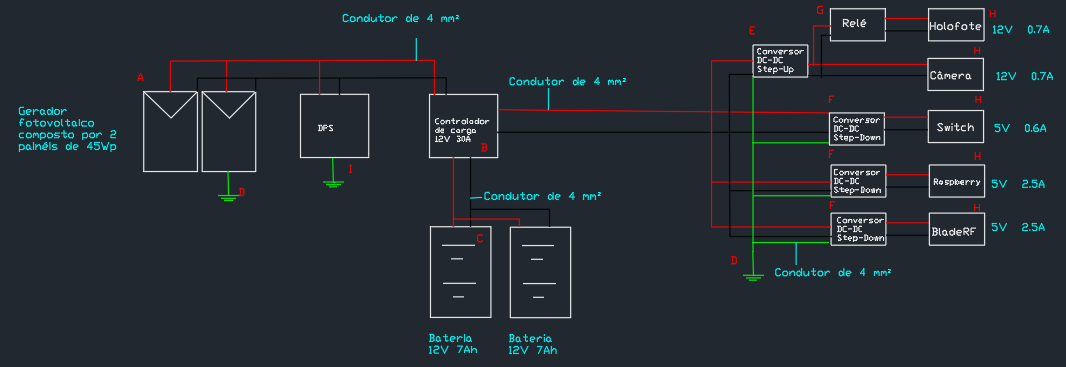
\includegraphics[scale=0.5]{DPS1.PNG}
\caption{Diagrama unifilar - AutoCad.}
\label{fig:diagrama}
\end{figure}



\subsection{Subsistema Energia}

O sistema de alimentação isolado do radar será apresentado na Figura \ref{fig:su}.

\begin{figure}[H]
\centering
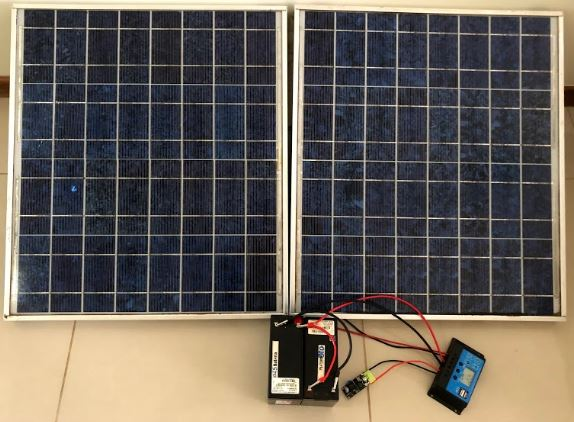
\includegraphics[scale=0.8]{subsis.JPG}

\caption{\label{fig:su}Sistema de alimentação do protótipo}
\end{figure}

O sistema é composto por 2 painéis fotovoltaicos da marca \textit{Kyocera} e capacidade de geração de 45 Wp cada um, duas baterias da marca \textit{Unipower} com capacidade de armazenamento de 7 Ah cada uma, um controlador de carga da marca \textit{Charge Controller} com limite de corrente de 30 A , 1 conversor DC-DC e um dispositivo de proteção contra surtos.

\subsection{Testes Subsistema Energia}

Foram realizados testes no sistema fotovoltaico e as tensões de saídas requeridas foram obtidas. Na Figura \ref{fig:teste} será apresentado um dos testes realizado para verificação da tensão.

\begin{figure}[H]
\centering
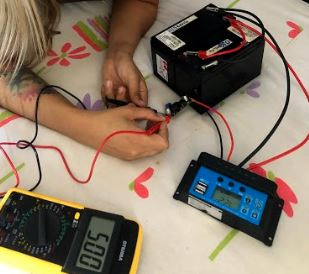
\includegraphics[scale=1.1]{teste.JPG}

\caption{\label{fig:teste}Teste de verificação de tensão do sistema de alimentação do protótipo}
\end{figure}


\subsection{Custos}

\begin{itemize}
    \item \textbf{Funcionamento do radar durante 24 horas por dia}
\end{itemize}

\begin{table}[H]
\begin{tabular}{|c|c|c|c|c|}
\hline
\multicolumn{5}{|c|}{Energia}                                                 \\ \hline
Material             & Preço         & Quantidade & Total         & Marca     \\ \hline
Painel Fotovoltaico  & R\$ 395,00  & 1          & R\$ 395,00  & UP SOLAR    \\ \hline
Bateria 70Ah             & R\$ 269,99  & 1          & R\$ 269,00  & Heliar  \\ \hline
Bateria 185Ah             & R\$ 1109,99  & 1          & R\$ 1109,99  & Heliar  \\ \hline
Controlador de Carga & R\$ 49,99  & 1          & R\$ 49,90  & charge controller \\ \hline
Lâmpada de LED       & R\$ 46,00 & 1          & R\$ 46,00 & PXT         \\ \hline
Conversor DC-DC       & R\$ 15,90 & 4          & R\$ 63,90 & Tenstar Robot         \\ \hline
Relé       & R\$ 9,90 & 1          & R\$ 9,90 & Eletrogate         \\ \hline
Total & - & - & 1943,69 & - \\ \hline
\end{tabular}
\end{table}



\begin{itemize}
    \item \textbf{Funcionamento do radar durante 3 horas por dia}
\end{itemize}
\begin{table}[H]
\begin{tabular}{|c|c|c|c|c|}
\hline
\multicolumn{5}{|c|}{Energia}                                                 \\ \hline
Material             & Preço         & Quantidade & Total         & Marca     \\ \hline
Lâmpada de LED       & R\$ 78,00 & 1          & R\$ 78,00 & PXT         \\ \hline
Conversor DC-DC       & R\$ 15,90 & 4          & R\$ 63,90 & Tenstar Robot         \\ \hline
Relé       & R\$ 9,90 & 1          & R\$ 9,90 & Eletrogate         \\ \hline
Total & - & - & R\$ 151,50 & - \\ \hline
\end{tabular}
\end{table}
